
\section{Descripción de la empresa}

PedidosNow es una empresa argentina fundada en 2010 que ofrece un servicio de gestión y seguimiento de pedidos de comida a domicilio. Desde su creación, se ha expandido a más de 20 países en Latinoamérica y cuenta con una base de más de 30 millones de usuarios, más de 15,000 cadenas de restaurantes afiliadas y aproximadamente 300,000 repartidores registrados. La empresa procesa más de 23 millones de pedidos anuales, con ingresos que superan los \$3,500 millones de dólares y una valuación en bolsa de \$35,000 millones de dólares.

El servicio de PedidosNow funciona a través de un sistema de software disponible en sitio web y aplicaciones móviles, que conecta a clientes, restaurantes y repartidores de manera eficiente. Los clientes pueden explorar restaurantes, realizar pedidos, pagar en línea y hacer seguimiento en tiempo real de sus envíos. Los restaurantes pueden registrar sus sucursales, cargar su menú, gestionar pedidos y acceder a estadísticas sobre su desempeño. Los repartidores, por su parte, pueden elegir sus horarios y zonas de trabajo, recibiendo incentivos financieros en función de la demanda.

Para optimizar la logística de entrega, PedidosNow asigna automáticamente cada pedido al repartidor y restaurante más convenientes, minimizando tiempos y costos de envío. Además, el sistema ofrece soporte a clientes, restaurantes y repartidores, garantizando la mejor experiencia posible a través de atención al cliente, gestión de reembolsos y resolución de problemas en los envíos.

La empresa se organiza en diferentes áreas clave: gerencia, tecnología y desarrollo de producto, operaciones y logística, marketing, recursos humanos, finanzas y legal, y atención al cliente. Cada una de estas áreas contribuye al crecimiento y éxito de la plataforma, asegurando una operación eficiente y en constante evolución.

\subsection{Actividades que realiza la empresa}

La actividad principal de la empresa es desarrollar y mantener un sistema de software, donde los clientes pueden realizar pedidos de comida a domicilio en más de 15,000 restaurantes, desde su computadora o dispositivo móvil. También permite a restaurantes registrarse y ofrecer sus productos a través de PedidosNow, y a sus repartidores registrados la capacidad de elegir sus horarios y zonas de trabajo. Para cumplir con esta misión, la empresa actúa como intermediaria entre tres tipos de entidades: clientes, restaurantes y repartidores.

La empresa, además, se encarga de la logística del reparto de los envíos, asignando cada orden realizada, al repartidor y a la sucursal (en caso de una cadena de restaurantes) más convenientes, según sus ubicaciones, horario de trabajo del repartidor, etc. El sistema busca evitar que el tiempo de los repartidores y restaurantes sea desaprovechado, a la vez que intenta minimizar el costo y tiempo de envío. Para ello, ofrece incentivos financieros a los repartidores, a través de comisiones más altas, para que elijan trabajar en las zonas geográficas y horarios con mayor demanda.

La empresa ofrece su servicio a través de un sitio web y aplicaciones móviles para iOS y Android. Tanto clientes, como restaurantes y repartidores, utilizan este sistema de software para interactuar con PedidosNow.

\subsubsection{Actividades relacionadas a los clientes}

Los clientes son los usuarios principales de la aplicación. El sistema cuenta con la capacidad de registrar clientes nuevos, y permite a los clientes ya registrados iniciar sesión. El cliente puede cargar distintas direcciones de envío para sus pedidos.

En la página principal, permite a los clientes explorar los distintos restaurantes que ofrecen sus productos a través de PedidosNow. El cliente puede observar los distintos productos de cada restaurante, sus precios y si hay stock disponible. De cada restaurante, se indican el tiempo estimado de entrega, costo de envío, horarios de atención, y reseñas y puntuaciones realizadas por otros usuarios.

El cliente tiene la posibilidad de agregar productos de un restaurante a su carrito de compras, siempre que el mismo se encuentre abierto y el producto en cuestión se encuentre en stock. Solo puede agregar productos de un mismo restaurante. Si el sistema detecta que el restaurante está muy lejos de la dirección de envío del cliente, le alertará que no podrá realizar la compra a menos que cambie su dirección a la hora de realizar la compra.

Una vez que el cliente ha agregado todos los productos que le interesan comprar al carrito, puede proceder con la compra. Primero debe indicar la dirección de envío, ya sea una cargada anteriormente, o una nueva. Si el restaurante se encuentra demasiado lejos, o no hay repartidores disponibles, no se podrá proceder con la compra. De lo contrario, solicita al usuario el medio de pago a utilizar, y el ingreso de los datos requeridos por el mismo (Nº de tarjeta, código de seguridad, etc.).

Si el pago es exitoso, se envía la orden a la sucursal más ideal para que comience su preparación, y se asigna el repartidor más conveniente para el reparto del pedido.

Una vez realizada la compra, el sistema ofrece al cliente la capacidad de realizar el rastreo y seguimiento de su pedido, indicándose el estado actual del mismo, detalles de la compra y el pago, detalles del repartidor asignado (nombre, ubicación), tiempo estimado de finalización, etc. El cliente no podrá realizar más de un pedido a la vez.

El cliente tiene un breve periodo de tiempo, antes de que el restaurante empiece a preparar la orden, para cancelarla. También puede hacerlo si el tiempo de envío excede por mucho el tiempo estimado al realizar la compra.

Si el envío es imposible de realizar debido a razones de fuerza mayor, se alerta al cliente que el envío fue cancelado y se le realiza un reembolso inmediato.

Por otro lado, si el envío es completado con éxito, el cliente puede dejar una puntuación y reseña del restaurante. También puede ver un historial de sus pedidos realizados anteriormente.

Si el cliente no está conforme con el envío, puede solicitar un reembolso a través de la aplicación.

\subsubsection{Actividades relacionadas a los restaurantes}

Cualquier restaurante habilitado en las ciudades donde opera PedidosNow puede registrarse con la empresa para ofrecer sus productos a través de la app. La carga de un restaurante nuevo no es completamente automática, sino que requiere verificación humana de la autenticidad del mismo y de su habilitación para operar.

Como condición para trabajar con la empresa, deben pagar como comisión cada mes un porcentaje de sus ingresos totales obtenidos a través de PedidosNow.

Las grandes cadenas de restaurantes pueden acceder a contratos más beneficiosos con comisiones más bajas, si cumplen con ciertos volúmenes de venta mínimos, o acuerdan no trabajar con servicios de reparto competidores.

El sistema permite a los dueños de los restaurantes cargar sus sucursales, productos (con sus precios, imágenes, descripción, tiempo de preparación, nivel de stock, etc.).

PedidosNow también ofrece a los restaurantes, estadísticas y analíticas de las ventas realizas, productos más buscados, y otros datos de utilidad para que los restaurantes puedan mejorar su servicios.

Si por alguna razón, se hiciese imposible la realización de una orden, el restaurante puede cancelar el pedido pero deberá pagar una multa a PedidosNow. En caso de acumular muchas faltas, PedidosNow terminará el contrato con el restaurante en cuestión.

\subsubsection{Actividades relacionadas a los repartidores}

La empresa ofrece a cualquier mayor de 18 años con un vehículo apto para reparto y un DNI válido la posibilidad de trabajar como repartidor en su servicio. Los interesados en ser repartidores deben registrarse como tal en la app, subir la documentación requerida, y esperar a ser aprobados por una verificación humana.

Cada repartidor recibe una comisión por cada pedido realizado con éxito.

Permite a los repartidores la capacidad de elegir sus horarios y zonas de trabajo, aunque ofrece de forma dinámica comisiones más altas en los horarios y zonas con más demanda de pedidos.

Durante el horario de trabajo, asigna a los repartidores los pedidos a realizar, indicándoles las direcciones de la sucursal de envío y el cliente, la ruta a seguir, detalles de la orden, y algunos datos del cliente.

Si el repartidor tiene un inconveniente de fuerza mayor al realizar el pedido, puede contactar a soporte a través de la app para intentar solucionarlo o cancelar el pedido, aunque no cobrará comisión. También puede cancelar el envío actual e incluso su turno de trabajo antes de tiempo, pero además de no cobrar comisión, será penalizado con multas y, en caso de acumular muchas faltas, terminación del contrato.


\subsection{Estructura de la empresa}

La empresa está organizada en las siguientes áreas:

\begin{itemize}
    \item \textbf{Gerencia} \nopagebreak
    
    Consiste de los ejecutivos de alto nivel, incluyendo al CEO, COO, CFO, CTO y CMO. Decide los objetivos y metas de la empresa, toma las decisiones de mayor responsabilidad, y realiza acuerdos de gran envergadura con otras empresas.

    \item \textbf{Tecnología y Desarrollo del Producto} \nopagebreak
    
    Encargada principalmente de mantener el software y la infraestructura de la empresa. También está encargada de la ciberseguridad y del análisis de datos. Se divide en los departamentos de Ingeniería y Desarrollo, Data Science y Machine Learning, Ciberseguridad y Compliance, y UX/UI y Diseño de Producto.

    \item \textbf{Operaciones y Logística} \nopagebreak
    
    Gestiona la flota de repartidores, optimiza rutas y tiempos de entrega, y supervisa la calidad del servicio para garantizar eficiencia y satisfacción del usuario. También provee soporte a los repartidores. Se divide en los departamentos de Gestión de Flota de Repartidores, Optimización de Rutas y Logística, Soporte a Repartidores, y Control de Calidad.

    \item \textbf{Comercial y Alianzas Estratégicas} \nopagebreak
    
    Se encarga de atraer y gestionar restaurantes y comercios, negociando condiciones, acuerdos y asegurando buenas relaciones con los socios comerciales. También provee soporte a los mismos. Se divide en los departamentos de Relaciones con Restaurantes y Comercios, Negociaciones y Contratos, y Atención a Socios Comerciales.

    \item \textbf{Marketing} \nopagebreak
    
    Responsable de las campañas de marketing, SEO, retención de usuarios, promociones, la identidad de la marca, uso de redes sociales, y análisis de mercado. Se divide en los departamentos de Adquisición de Usuarios, Marketing Digital y Redes Sociales, CRM (Customer Relationship Management) y Fidelización, e Inteligencia de Mercado.

    \item \textbf{Recursos Humanos} \nopagebreak
    
    Gestiona la contratación, bienestar y desarrollo del talento dentro de la empresa, asegurando un buen ambiente laboral y crecimiento profesional. Se divide en los departamentos de Reclutamiento y Selección, Capacitación y Desarrollo, y Bienestar y Cultura Organizacional.

    \item \textbf{Finanzas y Legal} \nopagebreak
    
    Administra pagos, inversiones y costos de la empresa, además de garantizar que todas las operaciones cumplan con las leyes y regulaciones locales. Se divide en los departamentos de Contabilidad y Facturación, Estrategia Financiera, y Legal y Compliance.

    \item \textbf{Atención al Cliente} \nopagebreak
    
    Provee soporte a clientes, restaurantes y repartidores, resolviendo problemas, reclamos y asegurando una buena experiencia en la plataforma. Se divide en los departamentos de Soporte al Usuario, Gestión de Reclamos y Reembolsos, y Mejora de la Experiencia.
\end{itemize}

\subsection{Organigrama de la empresa}
\begin{figure}[H]
    \centering
    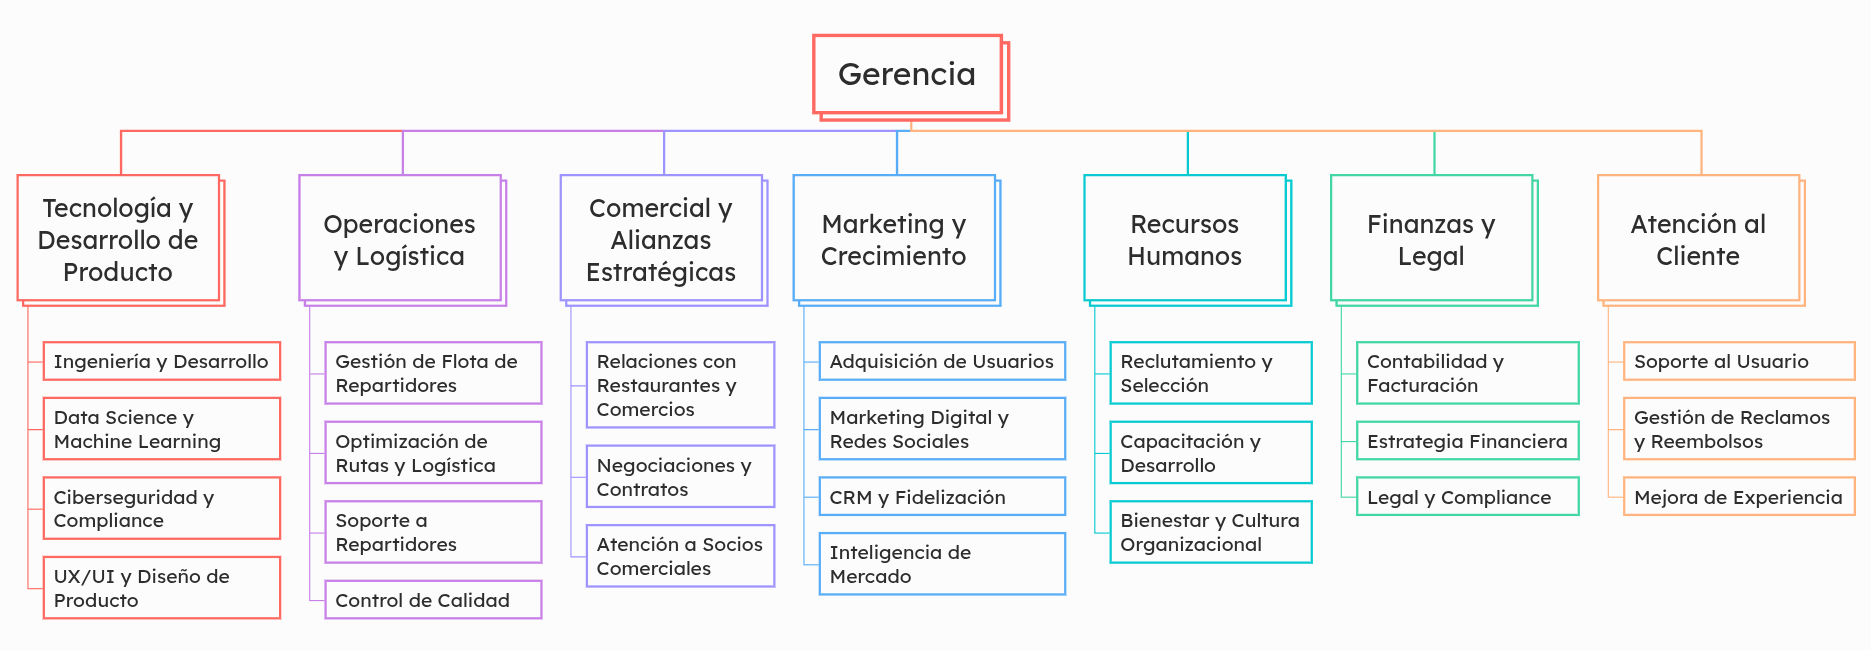
\includegraphics[width=\textwidth]{./img/organigrama.png}
    \caption{Organigrama de la empresa.}
\end{figure}